\documentclass[]{article}
\usepackage{lmodern}
\usepackage{amssymb,amsmath}
\usepackage{ifxetex,ifluatex}
\usepackage{fixltx2e} % provides \textsubscript
\ifnum 0\ifxetex 1\fi\ifluatex 1\fi=0 % if pdftex
  \usepackage[T1]{fontenc}
  \usepackage[utf8]{inputenc}
\else % if luatex or xelatex
  \ifxetex
    \usepackage{mathspec}
  \else
    \usepackage{fontspec}
  \fi
  \defaultfontfeatures{Ligatures=TeX,Scale=MatchLowercase}
\fi
% use upquote if available, for straight quotes in verbatim environments
\IfFileExists{upquote.sty}{\usepackage{upquote}}{}
% use microtype if available
\IfFileExists{microtype.sty}{%
\usepackage{microtype}
\UseMicrotypeSet[protrusion]{basicmath} % disable protrusion for tt fonts
}{}
\usepackage[margin=1in]{geometry}
\usepackage{hyperref}
\hypersetup{unicode=true,
            pdftitle={Patagonia parrots density analysis},
            pdfauthor={Francisco Dénes and Peter Sólymos},
            pdfborder={0 0 0},
            breaklinks=true}
\urlstyle{same}  % don't use monospace font for urls
\usepackage{color}
\usepackage{fancyvrb}
\newcommand{\VerbBar}{|}
\newcommand{\VERB}{\Verb[commandchars=\\\{\}]}
\DefineVerbatimEnvironment{Highlighting}{Verbatim}{commandchars=\\\{\}}
% Add ',fontsize=\small' for more characters per line
\usepackage{framed}
\definecolor{shadecolor}{RGB}{248,248,248}
\newenvironment{Shaded}{\begin{snugshade}}{\end{snugshade}}
\newcommand{\KeywordTok}[1]{\textcolor[rgb]{0.13,0.29,0.53}{\textbf{#1}}}
\newcommand{\DataTypeTok}[1]{\textcolor[rgb]{0.13,0.29,0.53}{#1}}
\newcommand{\DecValTok}[1]{\textcolor[rgb]{0.00,0.00,0.81}{#1}}
\newcommand{\BaseNTok}[1]{\textcolor[rgb]{0.00,0.00,0.81}{#1}}
\newcommand{\FloatTok}[1]{\textcolor[rgb]{0.00,0.00,0.81}{#1}}
\newcommand{\ConstantTok}[1]{\textcolor[rgb]{0.00,0.00,0.00}{#1}}
\newcommand{\CharTok}[1]{\textcolor[rgb]{0.31,0.60,0.02}{#1}}
\newcommand{\SpecialCharTok}[1]{\textcolor[rgb]{0.00,0.00,0.00}{#1}}
\newcommand{\StringTok}[1]{\textcolor[rgb]{0.31,0.60,0.02}{#1}}
\newcommand{\VerbatimStringTok}[1]{\textcolor[rgb]{0.31,0.60,0.02}{#1}}
\newcommand{\SpecialStringTok}[1]{\textcolor[rgb]{0.31,0.60,0.02}{#1}}
\newcommand{\ImportTok}[1]{#1}
\newcommand{\CommentTok}[1]{\textcolor[rgb]{0.56,0.35,0.01}{\textit{#1}}}
\newcommand{\DocumentationTok}[1]{\textcolor[rgb]{0.56,0.35,0.01}{\textbf{\textit{#1}}}}
\newcommand{\AnnotationTok}[1]{\textcolor[rgb]{0.56,0.35,0.01}{\textbf{\textit{#1}}}}
\newcommand{\CommentVarTok}[1]{\textcolor[rgb]{0.56,0.35,0.01}{\textbf{\textit{#1}}}}
\newcommand{\OtherTok}[1]{\textcolor[rgb]{0.56,0.35,0.01}{#1}}
\newcommand{\FunctionTok}[1]{\textcolor[rgb]{0.00,0.00,0.00}{#1}}
\newcommand{\VariableTok}[1]{\textcolor[rgb]{0.00,0.00,0.00}{#1}}
\newcommand{\ControlFlowTok}[1]{\textcolor[rgb]{0.13,0.29,0.53}{\textbf{#1}}}
\newcommand{\OperatorTok}[1]{\textcolor[rgb]{0.81,0.36,0.00}{\textbf{#1}}}
\newcommand{\BuiltInTok}[1]{#1}
\newcommand{\ExtensionTok}[1]{#1}
\newcommand{\PreprocessorTok}[1]{\textcolor[rgb]{0.56,0.35,0.01}{\textit{#1}}}
\newcommand{\AttributeTok}[1]{\textcolor[rgb]{0.77,0.63,0.00}{#1}}
\newcommand{\RegionMarkerTok}[1]{#1}
\newcommand{\InformationTok}[1]{\textcolor[rgb]{0.56,0.35,0.01}{\textbf{\textit{#1}}}}
\newcommand{\WarningTok}[1]{\textcolor[rgb]{0.56,0.35,0.01}{\textbf{\textit{#1}}}}
\newcommand{\AlertTok}[1]{\textcolor[rgb]{0.94,0.16,0.16}{#1}}
\newcommand{\ErrorTok}[1]{\textcolor[rgb]{0.64,0.00,0.00}{\textbf{#1}}}
\newcommand{\NormalTok}[1]{#1}
\usepackage{longtable,booktabs}
\usepackage{graphicx,grffile}
\makeatletter
\def\maxwidth{\ifdim\Gin@nat@width>\linewidth\linewidth\else\Gin@nat@width\fi}
\def\maxheight{\ifdim\Gin@nat@height>\textheight\textheight\else\Gin@nat@height\fi}
\makeatother
% Scale images if necessary, so that they will not overflow the page
% margins by default, and it is still possible to overwrite the defaults
% using explicit options in \includegraphics[width, height, ...]{}
\setkeys{Gin}{width=\maxwidth,height=\maxheight,keepaspectratio}
\IfFileExists{parskip.sty}{%
\usepackage{parskip}
}{% else
\setlength{\parindent}{0pt}
\setlength{\parskip}{6pt plus 2pt minus 1pt}
}
\setlength{\emergencystretch}{3em}  % prevent overfull lines
\providecommand{\tightlist}{%
  \setlength{\itemsep}{0pt}\setlength{\parskip}{0pt}}
\setcounter{secnumdepth}{0}
% Redefines (sub)paragraphs to behave more like sections
\ifx\paragraph\undefined\else
\let\oldparagraph\paragraph
\renewcommand{\paragraph}[1]{\oldparagraph{#1}\mbox{}}
\fi
\ifx\subparagraph\undefined\else
\let\oldsubparagraph\subparagraph
\renewcommand{\subparagraph}[1]{\oldsubparagraph{#1}\mbox{}}
\fi

%%% Use protect on footnotes to avoid problems with footnotes in titles
\let\rmarkdownfootnote\footnote%
\def\footnote{\protect\rmarkdownfootnote}

%%% Change title format to be more compact
\usepackage{titling}

% Create subtitle command for use in maketitle
\newcommand{\subtitle}[1]{
  \posttitle{
    \begin{center}\large#1\end{center}
    }
}

\setlength{\droptitle}{-2em}
  \title{Patagonia parrots density analysis}
  \pretitle{\vspace{\droptitle}\centering\huge}
  \posttitle{\par}
  \author{Francisco Dénes and Peter Sólymos}
  \preauthor{\centering\large\emph}
  \postauthor{\par}
  \predate{\centering\large\emph}
  \postdate{\par}
  \date{June 2, 2018}

\usepackage{float}

\begin{document}
\maketitle

\section{Motivation}\label{motivation}

We want to model the density of the austral parakeet \emph{Enicognathus
ferrugineus} and the slender-billed parakeet \emph{Enicognathus
leptorhynchus} from count data obtained with road transect surveys in
Patagonia. Because these parrots are gregarious, we want to assess
whether group size and size of groups vary across habitats and between
breeding (Nov-Dec) and non-breeding seasons (Jan-Oct). We use distance
sampling methods to account for detectability of parrots.

These animals tend to form smaller or larger groups, but groups of size
2 are also often observed as a result of mating pairs, as shown in
Figure 1.

\begin{figure}[H]
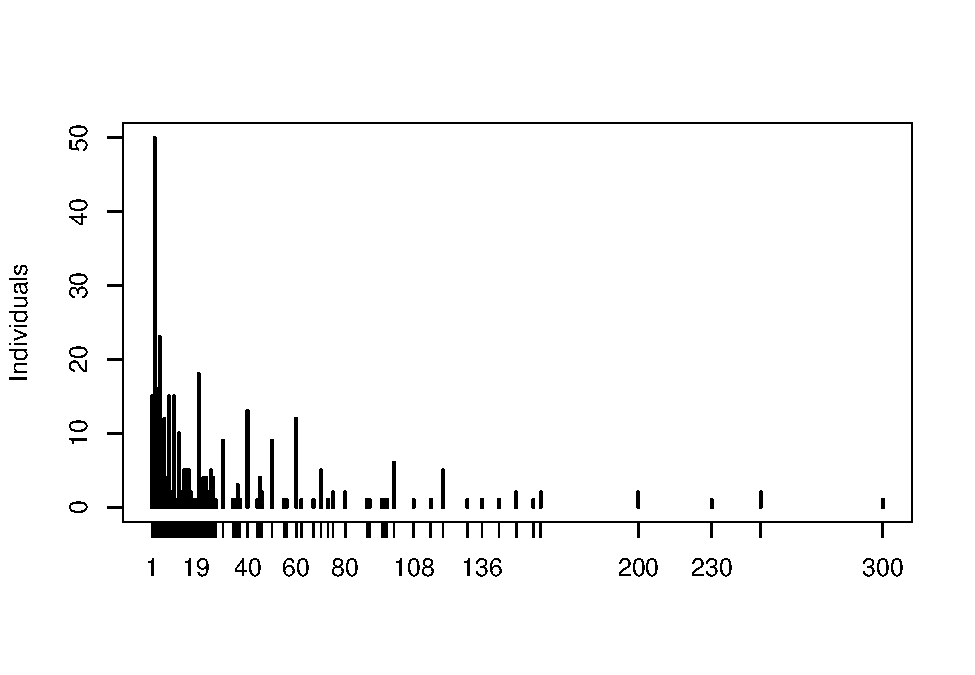
\includegraphics{Patagonia_parrots_density_analysis_files/figure-latex/unnamed-chunk-1-1} \caption{\textit{Enicognathus ferrugineus} count frequencies}\label{fig:unnamed-chunk-1}
\end{figure}

\section{\texorpdfstring{Austral parakeet \emph{Enicognathus
ferrugineus}}{Austral parakeet Enicognathus ferrugineus}}\label{austral-parakeet-enicognathus-ferrugineus}

\subsection{Estimating effective detection radius
(EDR)}\label{estimating-effective-detection-radius-edr}

We fit distance sampling models with detection predictor variables,
including the average group size, the number of groups that were
observed (to account for the possibility that grouping behaviour
influences detectability), and also habitat type. We used
forward-stepwise model selection, starting with single covariate models
and eliminating covariates that do not improve model parsimony
(i.e.~result in AIC lower than 2) in relation to the null model.

\begin{longtable}[]{@{}lrrr@{}}
\caption{\textit{E. ferrugineous} EDR models AIC}\tabularnewline
\toprule
& df & AIC & dAIC\tabularnewline
\midrule
\endfirsthead
\toprule
& df & AIC & dAIC\tabularnewline
\midrule
\endhead
EDR.habitatype & 3 & 1434.532 & 0.00\tabularnewline
EDR.null & 1 & 1438.166 & 3.63\tabularnewline
EDR.avggroupsize & 2 & 1439.144 & 4.61\tabularnewline
EDR.numbergroups & 2 & 1440.166 & 5.63\tabularnewline
\bottomrule
\end{longtable}

The model (\texttt{EDR.habitatype}) has the lowest AIC (Table 1),
indicating that habitat type affects the effective detection radius
(EDR) of \emph{Enicognathus ferrugineus}. Specifically, detection radius
is higher in agropastoral than urban and other habitats (Table 2). This
means that detectability is higher in agropastoral habitats, and also
that the area surveyed in a given sample unit is larger if the habitat
therein is agropastoral vs.~urban or other, presubably because it is
possible to see further in pastures and planted fields than in forest or
urban environments.

\begin{verbatim}
## 
## Call:
## cmulti(formula = Y | D ~ Urban + Agropastoral, data = X, type = "dis")
## 
## Distance Sampling (half-normal, circular area)
## Conditional Maximum Likelihood estimates
## 
## Coefficients:
##                      Estimate Std. Error z value Pr(>|z|)    
## log.tau_(Intercept)   4.58872    0.03844 119.365   <2e-16 ***
## log.tau_Urban         0.05744    0.05814   0.988   0.3232    
## log.tau_Agropastoral  0.26269    0.10278   2.556   0.0106 *  
## ---
## Signif. codes:  0 '***' 0.001 '**' 0.01 '*' 0.05 '.' 0.1 ' ' 1 
## 
## Log-likelihood: -714.3 
## BIC =  1444
\end{verbatim}

\begin{longtable}[]{@{}lr@{}}
\caption{\textit{E. ferrugineous} habitat-specific EDR
(m)}\tabularnewline
\toprule
Habitat & EDR\tabularnewline
\midrule
\endfirsthead
\toprule
Habitat & EDR\tabularnewline
\midrule
\endhead
Other & 98.36847\tabularnewline
Urban & 104.18432\tabularnewline
Agropastoral & 127.92056\tabularnewline
\bottomrule
\end{longtable}

\section{Models for number of groups}\label{models-for-number-of-groups}

We then model the number of groups as a function of covariates. The
model for number of groups is G\textsubscript{i} \textasciitilde{}
Poisson(D\textsubscript{i}A\textsubscript{i}), where D\textsubscript{i}
= covariates and A\textsubscript{i} = area sampled in site.
A\textsubscript{i} is calculated using the habitat-specific estimated
EDR, and is added to the model as an offset. We build a first set of
models to evaluate the effect of covariates related to habitat (habitat
type and elevation).

\begin{figure}[H]
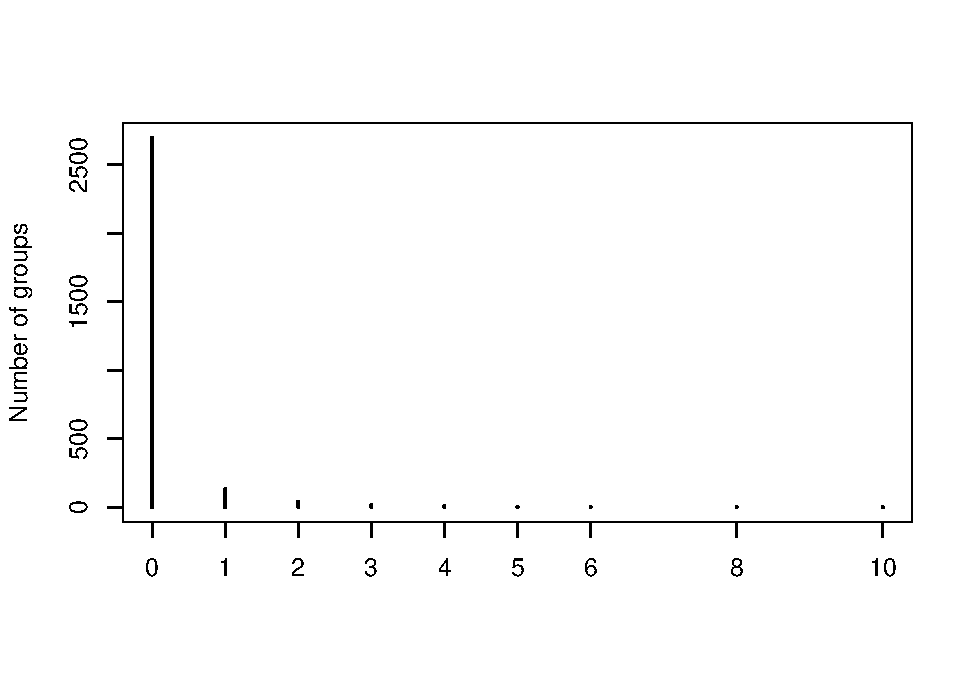
\includegraphics{Patagonia_parrots_density_analysis_files/figure-latex/unnamed-chunk-5-1} \caption{\textit{Enicognathus ferrugineus} group numbers }\label{fig:unnamed-chunk-5}
\end{figure}

\begin{longtable}[]{@{}lrrr@{}}
\caption{\textit{E. ferrugineous} number of group models}\tabularnewline
\toprule
& df & AIC & dAIC\tabularnewline
\midrule
\endfirsthead
\toprule
& df & AIC & dAIC\tabularnewline
\midrule
\endhead
ngroup.hab.ele2 & 5 & 2082.963 & 0.00\tabularnewline
ngroup.hab.ele & 4 & 2114.437 & 31.47\tabularnewline
ngroup.hab & 3 & 2133.717 & 50.75\tabularnewline
ngroup.ele2 & 3 & 2275.565 & 192.60\tabularnewline
ngroup.ele & 2 & 2323.806 & 240.84\tabularnewline
\bottomrule
\end{longtable}

\hfill\break

The model with both habitat type and elevation (quadratic effect) has
the lowest AIC (Table 3), indicating that both covariates affect the
number of groups:

\begin{verbatim}
## 
## Call:
## glm(formula = ngroups ~ habitat + elevation, family = poisson, 
##     data = sites, offset = log(sites$A))
## 
## Deviance Residuals: 
##     Min       1Q   Median       3Q      Max  
## -2.9552  -0.3696  -0.2192  -0.1266   7.6615  
## 
## Coefficients:
##                Estimate Std. Error z value Pr(>|z|)    
## (Intercept)  -3.8742985  0.2033144 -19.056  < 2e-16 ***
## habitatOther  1.7435771  0.1978580   8.812  < 2e-16 ***
## habitatUrban  2.4225361  0.2020368  11.991  < 2e-16 ***
## elevation    -0.0007506  0.0001637  -4.586 4.51e-06 ***
## ---
## Signif. codes:  0 '***' 0.001 '**' 0.01 '*' 0.05 '.' 0.1 ' ' 1
## 
## (Dispersion parameter for poisson family taken to be 1)
## 
##     Null deviance: 1865.3  on 2900  degrees of freedom
## Residual deviance: 1636.1  on 2897  degrees of freedom
## AIC: 2114.4
## 
## Number of Fisher Scoring iterations: 7
\end{verbatim}

\begin{verbatim}
## Analysis of Deviance Table
## 
## Model: poisson, link: log
## 
## Response: ngroups
## 
## Terms added sequentially (first to last)
## 
## 
##           Df Deviance Resid. Df Resid. Dev
## NULL                       2900     1865.3
## habitat    2  207.965      2898     1657.4
## elevation  1   21.279      2897     1636.1
\end{verbatim}

We then proceed by adding within-year temporal covariates
(breeding/non-breeding season and julian date) and their interactions
with habitat.

\begin{longtable}[]{@{}lrrr@{}}
\caption{\textit{E. ferrugineous} number of group models (within-year
temporal predictors) AIC}\tabularnewline
\toprule
& df & AIC & dAIC\tabularnewline
\midrule
\endfirsthead
\toprule
& df & AIC & dAIC\tabularnewline
\midrule
\endhead
ngroup.habXseason.ele & 8 & 2065.594 & 0.00\tabularnewline
ngroup.hab.ele.season & 6 & 2067.555 & 1.96\tabularnewline
ngroup.habXjdate.ele & 8 & 2081.546 & 15.95\tabularnewline
ngroup.hab.ele.jdate & 6 & 2084.491 & 18.90\tabularnewline
ngroup.hab.ele & 4 & 2114.437 & 48.84\tabularnewline
\bottomrule
\end{longtable}

Model with season*habitat interaction is equally parcimonious with the
model with only the additive effects. Given these are nested models,
this indicates the interaction only marginally improves the model fit,
so will continue with model with season and no interaction:

\subsubsection{season*habitat interaction
model}\label{seasonhabitat-interaction-model}

\begin{verbatim}
## 
## Call:
## glm(formula = ngroups ~ elevation + I(elevation^2) + habitat * 
##     season, family = poisson, data = sites, offset = log(sites$A))
## 
## Deviance Residuals: 
##     Min       1Q   Median       3Q      Max  
## -3.1791  -0.3703  -0.2113  -0.1192   7.9062  
## 
## Coefficients:
##                                   Estimate Std. Error z value Pr(>|z|)    
## (Intercept)                     -1.819e+01  5.580e+02  -0.033    0.974    
## elevation                       -3.900e-03  5.957e-04  -6.547 5.88e-11 ***
## I(elevation^2)                   2.637e-06  4.795e-07   5.500 3.80e-08 ***
## habitatOther                     1.580e+01  5.580e+02   0.028    0.977    
## habitatUrban                     2.008e+00  9.084e+02   0.002    0.998    
## seasonnon-breeding               1.519e+01  5.580e+02   0.027    0.978    
## habitatOther:seasonnon-breeding -1.436e+01  5.580e+02  -0.026    0.979    
## habitatUrban:seasonnon-breeding  2.663e-01  9.084e+02   0.000    1.000    
## ---
## Signif. codes:  0 '***' 0.001 '**' 0.01 '*' 0.05 '.' 0.1 ' ' 1
## 
## (Dispersion parameter for poisson family taken to be 1)
## 
##     Null deviance: 1865.3  on 2900  degrees of freedom
## Residual deviance: 1579.2  on 2893  degrees of freedom
## AIC: 2065.6
## 
## Number of Fisher Scoring iterations: 16
\end{verbatim}

\subsubsection{no interaction between season and
habitat}\label{no-interaction-between-season-and-habitat}

\begin{verbatim}
## 
## Call:
## glm(formula = ngroups ~ habitat + elevation + I(elevation^2) + 
##     season, family = poisson, data = sites, offset = log(sites$A))
## 
## Deviance Residuals: 
##     Min       1Q   Median       3Q      Max  
## -3.1472  -0.3692  -0.2153  -0.1244   7.8798  
## 
## Coefficients:
##                      Estimate Std. Error z value Pr(>|z|)    
## (Intercept)        -4.250e+00  4.119e-01 -10.318  < 2e-16 ***
## habitatOther        1.510e+00  2.037e-01   7.411 1.25e-13 ***
## habitatUrban        2.314e+00  2.026e-01  11.424  < 2e-16 ***
## elevation          -3.800e-03  5.929e-04  -6.408 1.47e-10 ***
## I(elevation^2)      2.565e-06  4.781e-07   5.365 8.11e-08 ***
## seasonnon-breeding  1.175e+00  3.404e-01   3.451 0.000558 ***
## ---
## Signif. codes:  0 '***' 0.001 '**' 0.01 '*' 0.05 '.' 0.1 ' ' 1
## 
## (Dispersion parameter for poisson family taken to be 1)
## 
##     Null deviance: 1865.3  on 2900  degrees of freedom
## Residual deviance: 1585.2  on 2895  degrees of freedom
## AIC: 2067.6
## 
## Number of Fisher Scoring iterations: 7
\end{verbatim}

Finally, we assess year effects by adding a year covariate (2013-2016).

\begin{longtable}[]{@{}lrrr@{}}
\caption{\textit{E. ferrugineous} number of group models (year
predictor) AIC table}\tabularnewline
\toprule
& df & AIC & dAIC\tabularnewline
\midrule
\endfirsthead
\toprule
& df & AIC & dAIC\tabularnewline
\midrule
\endhead
ngroup.hab.ele.season.year & 9 & 2022.265 & 0.00\tabularnewline
ngroup.hab.ele.season & 6 & 2067.555 & 45.29\tabularnewline
\bottomrule
\end{longtable}

The model with lowest AIC indicates that the number of groups is
affected by habitat ype, elevation, season (breeding/non breeding) and
year.

\begin{verbatim}
## 
## Call:
## glm(formula = ngroups ~ habitat + elevation + I(elevation^2) + 
##     season + as.factor(year), family = poisson, data = sites, 
##     offset = log(sites$A))
## 
## Deviance Residuals: 
##     Min       1Q   Median       3Q      Max  
## -2.6688  -0.4066  -0.2324  -0.1305   7.4851  
## 
## Coefficients:
##                       Estimate Std. Error z value Pr(>|z|)    
## (Intercept)         -4.716e+00  4.170e-01 -11.311  < 2e-16 ***
## habitatOther         1.739e+00  2.062e-01   8.434  < 2e-16 ***
## habitatUrban         2.460e+00  2.037e-01  12.075  < 2e-16 ***
## elevation           -3.430e-03  6.005e-04  -5.712 1.12e-08 ***
## I(elevation^2)       2.230e-06  4.860e-07   4.588 4.47e-06 ***
## seasonnon-breeding   1.022e+00  3.479e-01   2.939  0.00329 ** 
## as.factor(year)2014  9.236e-02  1.683e-01   0.549  0.58307    
## as.factor(year)2015  9.180e-01  1.614e-01   5.688 1.28e-08 ***
## as.factor(year)2016  6.115e-01  2.053e-01   2.979  0.00289 ** 
## ---
## Signif. codes:  0 '***' 0.001 '**' 0.01 '*' 0.05 '.' 0.1 ' ' 1
## 
## (Dispersion parameter for poisson family taken to be 1)
## 
##     Null deviance: 1865.3  on 2900  degrees of freedom
## Residual deviance: 1533.9  on 2892  degrees of freedom
## AIC: 2022.3
## 
## Number of Fisher Scoring iterations: 6
\end{verbatim}

\begin{verbatim}
## Analysis of Deviance Table
## 
## Model: poisson, link: log
## 
## Response: ngroups
## 
## Terms added sequentially (first to last)
## 
## 
##                 Df Deviance Resid. Df Resid. Dev
## NULL                             2900     1865.3
## habitat          2  207.965      2898     1657.4
## elevation        1   21.279      2897     1636.1
## I(elevation^2)   1   33.475      2896     1602.6
## season           1   17.408      2895     1585.2
## as.factor(year)  3   51.290      2892     1533.9
\end{verbatim}

\section{Models for group size}\label{models-for-group-size}

The count distribution is characterized with a spike at 2 (Figure 1),
and by the absence of 0s due to group size being conditional on having
\textgreater{}0 birds to consider it a group.

We start developing a general V-Inflated Poisson (VIP) model (``V''
stands for variable, in refence to the ``Z'' representing 0 in a
zero-inflated model, or ZIP), then we add the \textgreater{}0 condition.

\subsection{Maximum likelihood}\label{maximum-likelihood}

Let \(Y\) be a random variable, and \(y\) are observations, \(V\) is the
count value that has some extra probability mass (\(V=0\) is the ZIP
model), \(f(y; \lambda)\) is the Poisson density
(\(f(y; \lambda) = e^{-\lambda} \frac{\lambda^{y}}{y!}\)).

The V-Inflated density can be written as
\(P(Y=y) = \phi I(Y=V) + (1-\phi) f(y; \lambda)\) which is
\(\phi + (1-\phi) f(V; \lambda)\) when \(Y=V\) and
\((1-\phi) f(y; \lambda)\) otherwise.

R functions for the VIP model are presented at the end of this document.
Simulations are done to check the estimating procedure.

We define the extra probability mass at \texttt{V=2} to account for the
group size peak in pairs. The model is also truncated at 0, because
there are no groups with 0 individuals. We include habitat type as a
covariate for the count (Poisson) component, and compare models with and
without season (breeding/non-breeding) as a covariate for the
V-inflation probability.

\begin{longtable}[]{@{}lrrr@{}}
\caption{\textit{E. ferrugineous} Group size models AIC
table}\tabularnewline
\toprule
& df & AIC & dAIC\tabularnewline
\midrule
\endfirsthead
\toprule
& df & AIC & dAIC\tabularnewline
\midrule
\endhead
VIP.habitat.season & 331 & 32075.50 & 0.00\tabularnewline
VIP.habitat & 332 & 32085.51 & 10.01\tabularnewline
\bottomrule
\end{longtable}

\begin{verbatim}
## 
## Call:
## vip(Y = x$count, X = X, Z = Z, V = 2, offsetx = log(x$A), truncate = TRUE, 
##     hessian = TRUE, method = "SANN")
## 
## V-Inflated (Zero-Truncated) Poisson Model
## 
## Coefficients:
##                      Estimate Std. Error z value Pr(>|z|)    
## P_(Intercept)         1.00002    0.01898  52.686  < 2e-16 ***
## P_Urban               1.75433    0.02294  76.483  < 2e-16 ***
## P_Agropastoral        0.61163    0.03653  16.744  < 2e-16 ***
## V_(Intercept)         1.31556    0.81619   1.612    0.107    
## V_seasonnon-breeding -3.47379    0.83871  -4.142 3.45e-05 ***
## ---
## Signif. codes:  0 '***' 0.001 '**' 0.01 '*' 0.05 '.' 0.1 ' ' 1 
## 
## Log-likelihood: -1.571e+04 
## BIC = 3.334e+04
\end{verbatim}

The model with season is more parsimonious (Table 6). Estimated model
coefficients indicate that group sizes are larger in urban (\(\beta\) =
1.75) and agropastoral (\(\beta\) = 0.61) habitats when compared to
other natural habitats. Moreover, the probability of there being extra
pairs (i.e.~the V-inflation probability, \(\phi\)) is smaller in the
non-breeding season (\(\beta\) = -3.47).

\begin{center}\rule{0.5\linewidth}{\linethickness}\end{center}

\section{\texorpdfstring{Slender-billed parakeet \emph{Enicognathus
leptorhynchus}}{Slender-billed parakeet Enicognathus leptorhynchus}}\label{slender-billed-parakeet-enicognathus-leptorhynchus}

\begin{figure}[H]
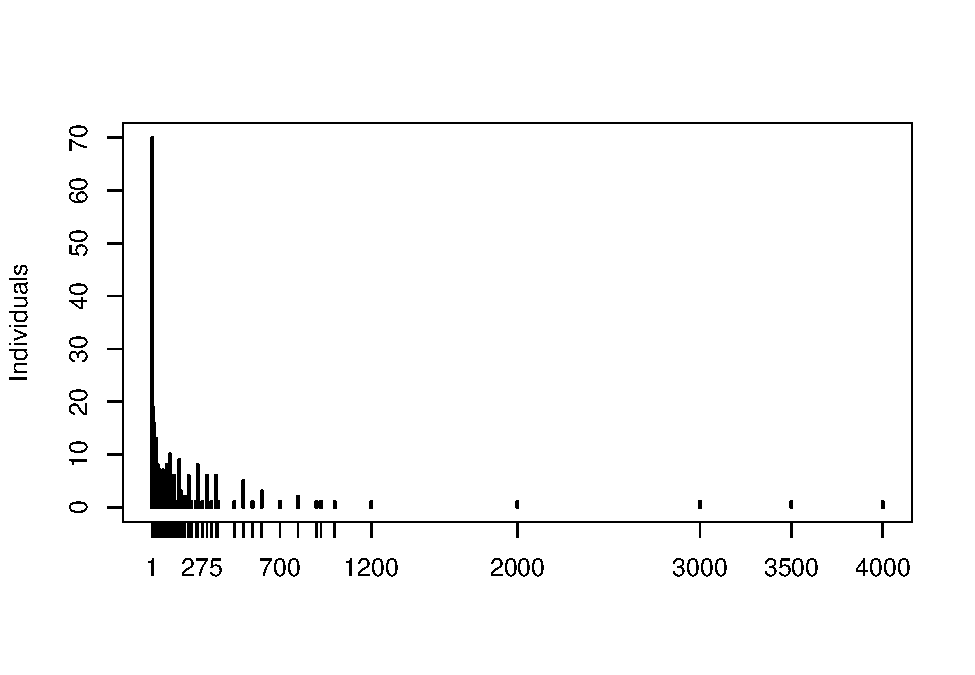
\includegraphics{Patagonia_parrots_density_analysis_files/figure-latex/unnamed-chunk-15-1} \caption{\textit{Enicognathus leptorhynchus} count frequencies}\label{fig:unnamed-chunk-15}
\end{figure}

\subsection{Estimating effective detection radius
(EDR)}\label{estimating-effective-detection-radius-edr-1}

\begin{longtable}[]{@{}lrrr@{}}
\caption{\textit{E. ferrugineous} EDR models AIC}\tabularnewline
\toprule
& df & AIC & dAIC\tabularnewline
\midrule
\endfirsthead
\toprule
& df & AIC & dAIC\tabularnewline
\midrule
\endhead
EDR.avggroupsize.habitat & 4 & 1054.464 & 0.00\tabularnewline
EDR.habitat.avggroupsize.numbergroups & 5 & 1059.062 &
4.60\tabularnewline
EDR.avggroupsize & 2 & 1063.875 & 9.41\tabularnewline
EDR.avggroupsize.numbergroups & 3 & 1064.553 & 10.09\tabularnewline
EDR.habitat.numbergroups & 4 & 1069.376 & 14.91\tabularnewline
EDR.habitatype & 3 & 1070.755 & 16.29\tabularnewline
EDR.null & 1 & 1086.330 & 31.87\tabularnewline
EDR.numbergroups & 2 & 1087.172 & 32.71\tabularnewline
\bottomrule
\end{longtable}

The model (\texttt{EDR.avggroupsize.habitat}) has the lowest AIC (Table
7), indicating that habitat type and average group size affect the
effective detection radius (EDR) of \emph{Enicognathus leptorhynchus}.
The mean EDR for each habitat, predicted using model coefficients and
the habitat-specific means of average group size, is shown in Table 8.

\begin{verbatim}
## 
## Call:
## cmulti(formula = Y | D ~ gavg + Urban + Agropastoral, data = X, 
##     type = "dis")
## 
## Distance Sampling (half-normal, circular area)
## Conditional Maximum Likelihood estimates
## 
## Coefficients:
##                        Estimate Std. Error    z value Pr(>|z|)    
## log.tau_(Intercept)   5.361e+00  4.209e-51  1.274e+51   <2e-16 ***
## log.tau_gavg          8.091e-04  8.419e-55  9.611e+50   <2e-16 ***
## log.tau_Urban        -2.655e-01  4.209e-51 -6.308e+49   <2e-16 ***
## log.tau_Agropastoral -2.883e-02  5.953e-51 -4.843e+48   <2e-16 ***
## ---
## Signif. codes:  0 '***' 0.001 '**' 0.01 '*' 0.05 '.' 0.1 ' ' 1 
## 
## Log-likelihood: -523.2 
## BIC =  1067
\end{verbatim}

\begin{longtable}[]{@{}lr@{}}
\caption{\textit{E. leptorhynchus} habitat-specific mean EDR
(m)}\tabularnewline
\toprule
Habitat & EDR\tabularnewline
\midrule
\endfirsthead
\toprule
Habitat & EDR\tabularnewline
\midrule
\endhead
Other & 235.4183\tabularnewline
Urban & 224.2124\tabularnewline
Agropastoral & 180.7002\tabularnewline
\bottomrule
\end{longtable}

\section{Models for number of
groups}\label{models-for-number-of-groups-1}

\begin{figure}[H]
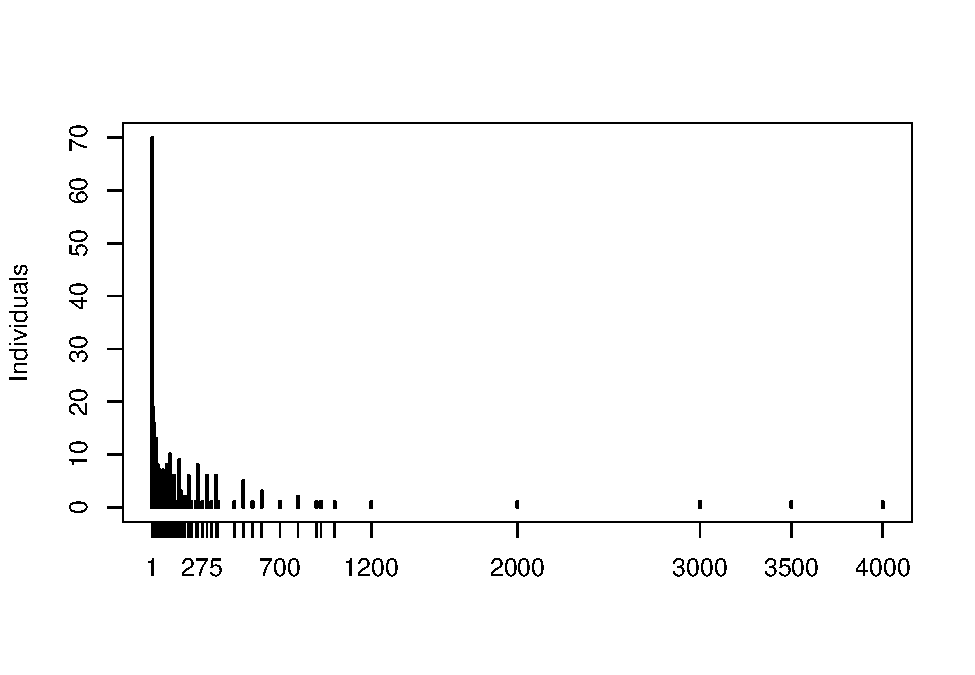
\includegraphics{Patagonia_parrots_density_analysis_files/figure-latex/unnamed-chunk-19-1} \caption{\textit{Enicognathus leptorhynchus} group numbers }\label{fig:unnamed-chunk-19}
\end{figure}

First set of models to evaluate the effect of covariates related to
habitat (habitat type and elevation):

\begin{longtable}[]{@{}lrrr@{}}
\caption{\textit{E. leptorhynchus} number of group
models}\tabularnewline
\toprule
& df & AIC & dAIC\tabularnewline
\midrule
\endfirsthead
\toprule
& df & AIC & dAIC\tabularnewline
\midrule
\endhead
ngroup.hab.ele2 & 5 & 2486.990 & -0.84\tabularnewline
ngroup.hab.ele & 4 & 2487.834 & 0.00\tabularnewline
ngroup.hab & 3 & 2493.346 & 5.51\tabularnewline
ngroup.ele2 & 3 & 2746.031 & 258.20\tabularnewline
ngroup.ele & 2 & 2761.122 & 273.29\tabularnewline
\bottomrule
\end{longtable}

The models with and habitat type and elevation (linear effect)habitat
type and elevation (quadratic effect) are equally parsimonious (Table
9). Given their nestedness, we drop the quadratic elevation effect and
continue with the model with habitat and linear elevation effects.

\begin{verbatim}
## 
## Call:
## glm(formula = ngroups ~ habitat + elevation, family = poisson, 
##     data = sites, offset = log(sites$A))
## 
## Deviance Residuals: 
##     Min       1Q   Median       3Q      Max  
## -4.7079  -0.4007  -0.2157  -0.1141  10.6088  
## 
## Coefficients:
##                Estimate Std. Error z value Pr(>|z|)    
## (Intercept)  -2.7809811  0.1232247 -22.568  < 2e-16 ***
## habitatOther -2.0346998  0.1466592 -13.874  < 2e-16 ***
## habitatUrban -0.7341155  0.1434994  -5.116 3.12e-07 ***
## elevation     0.0004781  0.0001748   2.736  0.00622 ** 
## ---
## Signif. codes:  0 '***' 0.001 '**' 0.01 '*' 0.05 '.' 0.1 ' ' 1
## 
## (Dispersion parameter for poisson family taken to be 1)
## 
##     Null deviance: 2358.9  on 2900  degrees of freedom
## Residual deviance: 2081.0  on 2897  degrees of freedom
## AIC: 2487.8
## 
## Number of Fisher Scoring iterations: 7
\end{verbatim}

\begin{verbatim}
## Analysis of Deviance Table
## 
## Model: poisson, link: log
## 
## Response: ngroups
## 
## Terms added sequentially (first to last)
## 
## 
##           Df Deviance Resid. Df Resid. Dev
## NULL                       2900     2358.9
## habitat    2  270.326      2898     2088.5
## elevation  1    7.512      2897     2081.0
\end{verbatim}

Adding within-year temporal covariates (breeding/non-breeding season and
julian date) and their interactions with habitat:

\begin{longtable}[]{@{}lrrr@{}}
\caption{\textit{E. leptorhynchus} number of group models (within-year
temporal predictors) AIC}\tabularnewline
\toprule
& df & AIC & dAIC\tabularnewline
\midrule
\endfirsthead
\toprule
& df & AIC & dAIC\tabularnewline
\midrule
\endhead
ngroup.habXjdate.ele & 7 & 2110.653 & 0.00\tabularnewline
ngroup.hab.ele.jdate & 5 & 2230.345 & 119.69\tabularnewline
ngroup.habXseason.ele & 7 & 2472.731 & 362.08\tabularnewline
ngroup.hab.ele & 4 & 2487.834 & 377.18\tabularnewline
ngroup.hab.ele.season & 5 & 2489.059 & 378.41\tabularnewline
\bottomrule
\end{longtable}

The model with jdate*habitat interaction has the lowest AIC (Table 9).

\subsubsection{season*habitat interaction
model}\label{seasonhabitat-interaction-model-1}

\begin{verbatim}
## 
## Call:
## glm(formula = ngroups ~ elevation + habitat * jdate, family = poisson, 
##     data = sites, offset = log(sites$A))
## 
## Deviance Residuals: 
##     Min       1Q   Median       3Q      Max  
## -4.6867  -0.3765  -0.0688  -0.0037   9.0194  
## 
## Coefficients:
##                      Estimate Std. Error z value Pr(>|z|)    
## (Intercept)        -1.4633740  0.1674177  -8.741  < 2e-16 ***
## elevation           0.0003340  0.0001723   1.939 0.052549 .  
## habitatOther        2.2340994  0.5897471   3.788 0.000152 ***
## habitatUrban        0.4120594  0.3099620   1.329 0.183720    
## jdate              -0.0057427  0.0005726 -10.029  < 2e-16 ***
## habitatOther:jdate -0.0399419  0.0071459  -5.589 2.28e-08 ***
## habitatUrban:jdate -0.0093727  0.0022889  -4.095 4.22e-05 ***
## ---
## Signif. codes:  0 '***' 0.001 '**' 0.01 '*' 0.05 '.' 0.1 ' ' 1
## 
## (Dispersion parameter for poisson family taken to be 1)
## 
##     Null deviance: 2358.9  on 2900  degrees of freedom
## Residual deviance: 1697.8  on 2894  degrees of freedom
## AIC: 2110.7
## 
## Number of Fisher Scoring iterations: 10
\end{verbatim}

Assess year effects by adding a year covariate (2013-2016).

\begin{longtable}[]{@{}lrrr@{}}
\caption{\textit{E. leptorhynchus} number of group models (year
predictor) AIC table}\tabularnewline
\toprule
& df & AIC & dAIC\tabularnewline
\midrule
\endfirsthead
\toprule
& df & AIC & dAIC\tabularnewline
\midrule
\endhead
ngroup.habXjdate.ele.year & 8 & 1993.981 & 0.00\tabularnewline
ngroup.habXjdate.ele & 7 & 2110.653 & 116.67\tabularnewline
\bottomrule
\end{longtable}

The model with lowest AIC indicates that the number of groups is
affected by habitat type, elevation, julian date and year.

\begin{verbatim}
## 
## Call:
## glm(formula = ngroups ~ habitat + elevation + season + as.factor(year), 
##     family = poisson, data = sites, offset = log(sites$A))
## 
## Deviance Residuals: 
##     Min       1Q   Median       3Q      Max  
## -2.9000  -0.4038  -0.2032  -0.1057   8.6857  
## 
## Coefficients:
##                       Estimate Std. Error z value Pr(>|z|)    
## (Intercept)         -3.9524864  0.2639635 -14.974  < 2e-16 ***
## habitatOther        -1.6293917  0.1495803 -10.893  < 2e-16 ***
## habitatUrban        -0.5062433  0.1443452  -3.507 0.000453 ***
## elevation            0.0004645  0.0001629   2.851 0.004355 ** 
## seasonnon-breeding  -0.7487438  0.2010999  -3.723 0.000197 ***
## as.factor(year)2014  0.6694517  0.2764278   2.422 0.015444 *  
## as.factor(year)2015  1.7634765  0.2366430   7.452 9.19e-14 ***
## as.factor(year)2016  3.2799760  0.2393254  13.705  < 2e-16 ***
## ---
## Signif. codes:  0 '***' 0.001 '**' 0.01 '*' 0.05 '.' 0.1 ' ' 1
## 
## (Dispersion parameter for poisson family taken to be 1)
## 
##     Null deviance: 2358.9  on 2900  degrees of freedom
## Residual deviance: 1579.2  on 2893  degrees of freedom
## AIC: 1994
## 
## Number of Fisher Scoring iterations: 7
\end{verbatim}

\begin{verbatim}
## Analysis of Deviance Table
## 
## Model: poisson, link: log
## 
## Response: ngroups
## 
## Terms added sequentially (first to last)
## 
## 
##                 Df Deviance Resid. Df Resid. Dev
## NULL                             2900     2358.9
## habitat          2   270.33      2898     2088.5
## elevation        1     7.51      2897     2081.0
## season           1     0.78      2896     2080.2
## as.factor(year)  3   501.08      2893     1579.2
\end{verbatim}

\section{Models for group size}\label{models-for-group-size-1}

\begin{verbatim}
##      P_(Intercept)     P_Urban P_Agropastoral V_(Intercept)
## [1,]    -3.4315607 24.02749982      17.308699     5.5023551
## [2,]    -1.6055318  5.64347167     -17.089005    13.1416174
## [3,]   -23.5915496 23.21956971      -6.478753    10.3184573
## [4,]     0.9674519  5.99061566       6.542012    16.3476814
## [5,]   -32.3644298 -0.01516136     -13.319216     0.8403038
## [6,]   -15.0687507 18.07756751       4.587351    49.1140564
##      V_seasonnon-breeding
## [1,]             11.61975
## [2,]             25.88478
## [3,]             30.86020
## [4,]             15.35033
## [5,]             43.74769
## [6,]             26.71279
\end{verbatim}

\begin{longtable}[]{@{}llrr@{}}
\toprule
& & 5\% & 95\%\tabularnewline
\midrule
\endhead
P\_(Intercept) & 15.5148542 & -34.103307 & 7.173057\tabularnewline
P\_Urban & -8.6162679 & -11.783613 & 28.778820\tabularnewline
P\_Agropastoral & -0.0262193 & -20.672452 & 19.980277\tabularnewline
V\_(Intercept) & -23.5420846 & 4.795528 & 45.179416\tabularnewline
V\_seasonnon-breeding & -22.8068590 & 1.472501 &
46.768732\tabularnewline
\bottomrule
\end{longtable}

\begin{center}\rule{0.5\linewidth}{\linethickness}\end{center}

\section{VIP model - R functions and
simulations}\label{vip-model---r-functions-and-simulations}

\begin{Shaded}
\begin{Highlighting}[]
\NormalTok{vip <-}
\ControlFlowTok{function}\NormalTok{(Y, X, Z, }\DataTypeTok{V=}\DecValTok{0}\NormalTok{,}
\NormalTok{offsetx, offsetz, weights, }\DataTypeTok{linkz=}\StringTok{"logit"}\NormalTok{,}
\DataTypeTok{truncate=}\OtherTok{FALSE}\NormalTok{, }\DataTypeTok{hessian=}\OtherTok{TRUE}\NormalTok{, }\DataTypeTok{method=}\StringTok{"Nelder-Mead"}\NormalTok{, }\DataTypeTok{init=}\OtherTok{NULL}\NormalTok{, ...) \{}
    \ControlFlowTok{if}\NormalTok{ (}\KeywordTok{missing}\NormalTok{(Y))}
        \KeywordTok{stop}\NormalTok{(}\StringTok{"C'mon, you must have some data?!"}\NormalTok{)}
    \ControlFlowTok{if}\NormalTok{ (truncate }\OperatorTok{&&}\StringTok{ }\KeywordTok{any}\NormalTok{(Y }\OperatorTok{<}\StringTok{ }\DecValTok{1}\NormalTok{))}
        \KeywordTok{stop}\NormalTok{(}\StringTok{"Y must be >0 when truncate=TRUE"}\NormalTok{)}
\NormalTok{    n <-}\StringTok{ }\KeywordTok{length}\NormalTok{(Y)}
\NormalTok{    id0 <-}\StringTok{ }\NormalTok{Y }\OperatorTok{==}\StringTok{ }\NormalTok{V}
\NormalTok{    id1 <-}\StringTok{ }\OperatorTok{!}\NormalTok{id0}
    \ControlFlowTok{if}\NormalTok{ (}\KeywordTok{missing}\NormalTok{(X)) \{}
\NormalTok{        X <-}\StringTok{ }\KeywordTok{matrix}\NormalTok{(}\DecValTok{1}\NormalTok{, n, }\DecValTok{1}\NormalTok{)}
        \KeywordTok{colnames}\NormalTok{(X) <-}\StringTok{ "(Intercept)"}
\NormalTok{    \}}
    \ControlFlowTok{if}\NormalTok{ (}\KeywordTok{missing}\NormalTok{(Z)) \{}
\NormalTok{        Z <-}\StringTok{ }\KeywordTok{matrix}\NormalTok{(}\DecValTok{1}\NormalTok{, n, }\DecValTok{1}\NormalTok{)}
        \KeywordTok{colnames}\NormalTok{(Z) <-}\StringTok{ "(Intercept)"}
\NormalTok{    \}}
\NormalTok{    kx <-}\StringTok{ }\KeywordTok{ncol}\NormalTok{(X)}
\NormalTok{    kz <-}\StringTok{ }\KeywordTok{ncol}\NormalTok{(Z)}
    \ControlFlowTok{if}\NormalTok{ (}\KeywordTok{missing}\NormalTok{(offsetx))}
\NormalTok{        offsetx <-}\StringTok{ }\DecValTok{0}
    \ControlFlowTok{if}\NormalTok{ (}\KeywordTok{missing}\NormalTok{(offsetz))}
\NormalTok{        offsetz <-}\StringTok{ }\DecValTok{0}
    \ControlFlowTok{if}\NormalTok{ (}\KeywordTok{missing}\NormalTok{(weights))}
\NormalTok{        weights <-}\StringTok{ }\KeywordTok{rep}\NormalTok{(}\DecValTok{1}\NormalTok{, n)}
\NormalTok{    linkinvx <-}\StringTok{ }\KeywordTok{poisson}\NormalTok{(}\StringTok{"log"}\NormalTok{)}\OperatorTok{$}\NormalTok{linkinv}
\NormalTok{    linkinvz <-}\StringTok{ }\KeywordTok{binomial}\NormalTok{(linkz)}\OperatorTok{$}\NormalTok{linkinv}
\NormalTok{    good.num.limit <-}\StringTok{ }\KeywordTok{c}\NormalTok{(.Machine}\OperatorTok{$}\NormalTok{double.xmin, .Machine}\OperatorTok{$}\NormalTok{double.xmax)}\OperatorTok{^}\NormalTok{(}\DecValTok{1}\OperatorTok{/}\DecValTok{3}\NormalTok{)}

\NormalTok{    ## VIP model full likelihood}
\NormalTok{    nll_VIP_ML <-}\StringTok{ }\ControlFlowTok{function}\NormalTok{(parms) \{}
\NormalTok{        mu <-}\StringTok{ }\KeywordTok{as.vector}\NormalTok{(}\KeywordTok{linkinvx}\NormalTok{(X }\OperatorTok\StringTok{ }\NormalTok{parms[}\DecValTok{1}\OperatorTok{:}\NormalTok{kx] }\OperatorTok{+}\StringTok{ }\NormalTok{offsetx))}
\NormalTok{        phi <-}\StringTok{ }\KeywordTok{as.vector}\NormalTok{(}\KeywordTok{linkinvz}\NormalTok{(Z }\OperatorTok\StringTok{ }\NormalTok{parms[(kx }\OperatorTok{+}\StringTok{ }\DecValTok{1}\NormalTok{)}\OperatorTok{:}\NormalTok{(kx }\OperatorTok{+}\StringTok{ }\NormalTok{kz)] }\OperatorTok{+}\StringTok{ }\NormalTok{offsetz))}
\NormalTok{        loglik0 <-}\StringTok{ }\KeywordTok{log}\NormalTok{(phi }\OperatorTok{+}\StringTok{ }\NormalTok{(}\DecValTok{1} \OperatorTok{-}\StringTok{ }\NormalTok{phi) }\OperatorTok{*}\StringTok{ }\KeywordTok{dpois}\NormalTok{(V, }\DataTypeTok{lambda =}\NormalTok{ mu, }\DataTypeTok{log =} \OtherTok{FALSE}\NormalTok{))}
\NormalTok{        loglik1 <-}\StringTok{ }\KeywordTok{log}\NormalTok{(}\DecValTok{1} \OperatorTok{-}\StringTok{ }\NormalTok{phi) }\OperatorTok{+}\StringTok{ }\KeywordTok{dpois}\NormalTok{(Y, }\DataTypeTok{lambda =}\NormalTok{ mu, }\DataTypeTok{log =} \OtherTok{TRUE}\NormalTok{)}
\NormalTok{        loglik <-}\StringTok{ }\KeywordTok{sum}\NormalTok{(weights[id0] }\OperatorTok{*}\StringTok{ }\NormalTok{loglik0[id0]) }\OperatorTok{+}\StringTok{ }\KeywordTok{sum}\NormalTok{(weights[id1] }\OperatorTok{*}\StringTok{ }\NormalTok{loglik1[id1])}
        \ControlFlowTok{if}\NormalTok{ (}\OperatorTok{!}\KeywordTok{is.finite}\NormalTok{(loglik) }\OperatorTok{||}\StringTok{ }\KeywordTok{is.na}\NormalTok{(loglik))}
\NormalTok{            loglik <-}\StringTok{ }\OperatorTok{-}\NormalTok{good.num.limit[}\DecValTok{2}\NormalTok{]}
        \OperatorTok{-}\NormalTok{loglik}
\NormalTok{    \}}
\NormalTok{    ## 0-truncated VIP model full likelihood}
\NormalTok{    nll_VIP_TR <-}\StringTok{ }\ControlFlowTok{function}\NormalTok{(parms) \{}
\NormalTok{        mu <-}\StringTok{ }\KeywordTok{as.vector}\NormalTok{(}\KeywordTok{linkinvx}\NormalTok{(X }\OperatorTok\StringTok{ }\NormalTok{parms[}\DecValTok{1}\OperatorTok{:}\NormalTok{kx] }\OperatorTok{+}\StringTok{ }\NormalTok{offsetx))}
\NormalTok{        phi <-}\StringTok{ }\KeywordTok{as.vector}\NormalTok{(}\KeywordTok{linkinvz}\NormalTok{(Z }\OperatorTok\StringTok{ }\NormalTok{parms[(kx }\OperatorTok{+}\StringTok{ }\DecValTok{1}\NormalTok{)}\OperatorTok{:}\NormalTok{(kx }\OperatorTok{+}\StringTok{ }\NormalTok{kz)] }\OperatorTok{+}\StringTok{ }\NormalTok{offsetz))}
\NormalTok{        loglik0 <-}\StringTok{ }\KeywordTok{log}\NormalTok{(phi }\OperatorTok{+}\StringTok{ }\NormalTok{(}\DecValTok{1} \OperatorTok{-}\StringTok{ }\NormalTok{phi) }\OperatorTok{*}\StringTok{ }\KeywordTok{dpois}\NormalTok{(V, }\DataTypeTok{lambda =}\NormalTok{ mu, }\DataTypeTok{log =} \OtherTok{FALSE}\NormalTok{) }\OperatorTok{/}\StringTok{ }\NormalTok{(}\DecValTok{1}\OperatorTok{-}\KeywordTok{exp}\NormalTok{(}\OperatorTok{-}\NormalTok{mu)))}
\NormalTok{        loglik1 <-}\StringTok{ }\KeywordTok{log}\NormalTok{((}\DecValTok{1} \OperatorTok{-}\StringTok{ }\NormalTok{phi) }\OperatorTok{*}\StringTok{ }\KeywordTok{dpois}\NormalTok{(Y, }\DataTypeTok{lambda =}\NormalTok{ mu, }\DataTypeTok{log =} \OtherTok{FALSE}\NormalTok{) }\OperatorTok{/}\StringTok{ }\NormalTok{(}\DecValTok{1}\OperatorTok{-}\KeywordTok{exp}\NormalTok{(}\OperatorTok{-}\NormalTok{mu)))}
\NormalTok{        loglik <-}\StringTok{ }\KeywordTok{sum}\NormalTok{(weights[id0] }\OperatorTok{*}\StringTok{ }\NormalTok{loglik0[id0]) }\OperatorTok{+}\StringTok{ }\KeywordTok{sum}\NormalTok{(weights[id1] }\OperatorTok{*}\StringTok{ }\NormalTok{loglik1[id1])}
        \ControlFlowTok{if}\NormalTok{ (}\OperatorTok{!}\KeywordTok{is.finite}\NormalTok{(loglik) }\OperatorTok{||}\StringTok{ }\KeywordTok{is.na}\NormalTok{(loglik))}
\NormalTok{            loglik <-}\StringTok{ }\OperatorTok{-}\NormalTok{good.num.limit[}\DecValTok{2}\NormalTok{]}
        \OperatorTok{-}\NormalTok{loglik}
\NormalTok{    \}}

    \ControlFlowTok{if}\NormalTok{ (}\KeywordTok{is.null}\NormalTok{(init))}
\NormalTok{      init <-}\StringTok{ }\KeywordTok{rep}\NormalTok{(}\DecValTok{0}\NormalTok{, kx}\OperatorTok{+}\NormalTok{kz)}
\NormalTok{    opt <-}\StringTok{ }\KeywordTok{optim}\NormalTok{(init, }
        \ControlFlowTok{if}\NormalTok{ (truncate) nll_VIP_TR }\ControlFlowTok{else}\NormalTok{ nll_VIP_ML, }
        \DataTypeTok{hessian=}\NormalTok{hessian, }\DataTypeTok{method=}\NormalTok{method, ...)}
\NormalTok{    par <-}\StringTok{ }\NormalTok{opt}\OperatorTok{$}\NormalTok{par}
    \KeywordTok{names}\NormalTok{(par) <-}\StringTok{ }\KeywordTok{c}\NormalTok{(}\KeywordTok{paste0}\NormalTok{(}\StringTok{"P_"}\NormalTok{, }\KeywordTok{colnames}\NormalTok{(X)), }\KeywordTok{paste0}\NormalTok{(}\StringTok{"V_"}\NormalTok{, }\KeywordTok{colnames}\NormalTok{(Z)))}
\NormalTok{    vc <-}\StringTok{ }\ControlFlowTok{if}\NormalTok{ (hessian)}
        \KeywordTok{solve}\NormalTok{(opt}\OperatorTok{$}\NormalTok{hessian) }\ControlFlowTok{else} \KeywordTok{matrix}\NormalTok{(}\OtherTok{NA}\NormalTok{, }\KeywordTok{length}\NormalTok{(par), }\KeywordTok{length}\NormalTok{(par))}
    \KeywordTok{dimnames}\NormalTok{(vc) <-}\StringTok{ }\KeywordTok{list}\NormalTok{(}\KeywordTok{names}\NormalTok{(par), }\KeywordTok{names}\NormalTok{(par))}
\NormalTok{    out <-}\StringTok{ }\KeywordTok{list}\NormalTok{(}\DataTypeTok{call=}\KeywordTok{match.call}\NormalTok{(),}
        \DataTypeTok{coefficients=}\NormalTok{par, }\DataTypeTok{loglik=}\OperatorTok{-}\NormalTok{opt}\OperatorTok{$}\NormalTok{value, }\DataTypeTok{vcov=}\NormalTok{vc, }\DataTypeTok{nobs=}\NormalTok{n,}
        \DataTypeTok{truncate=}\NormalTok{truncate)}
    \KeywordTok{class}\NormalTok{(out) <-}\StringTok{ "vip"}
\NormalTok{    out}
\NormalTok{\}}
\NormalTok{vcov.vip <-}\StringTok{ }\ControlFlowTok{function}\NormalTok{(object, ...) object}\OperatorTok{$}\NormalTok{vcov}
\NormalTok{logLik.vip <-}\StringTok{ }\ControlFlowTok{function}\NormalTok{ (object, ...)}
    \KeywordTok{structure}\NormalTok{(object}\OperatorTok{$}\NormalTok{loglik, }\DataTypeTok{df =}\NormalTok{ object}\OperatorTok{$}\NormalTok{nobs }\OperatorTok{-}\StringTok{ }\KeywordTok{length}\NormalTok{(object}\OperatorTok{$}\NormalTok{coef),}
        \DataTypeTok{nobs =}\NormalTok{ object}\OperatorTok{$}\NormalTok{nobs, }\DataTypeTok{class =} \StringTok{"logLik"}\NormalTok{)}
\NormalTok{summary.vip <-}\StringTok{ }\ControlFlowTok{function}\NormalTok{ (object, ...) \{}
\NormalTok{    k <-}\StringTok{ }\KeywordTok{length}\NormalTok{(object}\OperatorTok{$}\NormalTok{coefficients)}
\NormalTok{    coefs <-}\StringTok{ }\KeywordTok{coef}\NormalTok{(object)}
\NormalTok{    se <-}\StringTok{ }\KeywordTok{sqrt}\NormalTok{(}\KeywordTok{diag}\NormalTok{(}\KeywordTok{vcov}\NormalTok{(object)))}
\NormalTok{    tstat <-}\StringTok{ }\NormalTok{coefs}\OperatorTok{/}\NormalTok{se}
\NormalTok{    pval <-}\StringTok{ }\DecValTok{2} \OperatorTok{*}\StringTok{ }\KeywordTok{pnorm}\NormalTok{(}\OperatorTok{-}\KeywordTok{abs}\NormalTok{(tstat))}
\NormalTok{    coefs <-}\StringTok{ }\KeywordTok{cbind}\NormalTok{(coefs, se, tstat, pval)}
    \KeywordTok{colnames}\NormalTok{(coefs) <-}\StringTok{ }\KeywordTok{c}\NormalTok{(}\StringTok{"Estimate"}\NormalTok{, }\StringTok{"Std. Error"}\NormalTok{, }\StringTok{"z value"}\NormalTok{, }\StringTok{"Pr(>|z|)"}\NormalTok{)}
\NormalTok{    coefs <-}\StringTok{ }\NormalTok{coefs[}\DecValTok{1}\OperatorTok{:}\NormalTok{k, , drop =}\StringTok{ }\OtherTok{FALSE}\NormalTok{]}
    \KeywordTok{rownames}\NormalTok{(coefs) <-}\StringTok{ }\KeywordTok{names}\NormalTok{(}\KeywordTok{coef}\NormalTok{(object))}
\NormalTok{    out <-}\StringTok{ }\KeywordTok{list}\NormalTok{(}\DataTypeTok{call =}\NormalTok{ object}\OperatorTok{$}\NormalTok{call, }\DataTypeTok{coefficients=}\NormalTok{coefs, }\DataTypeTok{loglik =}\NormalTok{ object}\OperatorTok{$}\NormalTok{loglik,}
        \DataTypeTok{bic=}\KeywordTok{BIC}\NormalTok{(object), }\DataTypeTok{truncate=}\NormalTok{object}\OperatorTok{$}\NormalTok{truncate)}
    \KeywordTok{class}\NormalTok{(out) <-}\StringTok{ "summary.vip"}
    \KeywordTok{return}\NormalTok{(out)}
\NormalTok{\}}
\NormalTok{print.summary.vip <-}\StringTok{ }\ControlFlowTok{function}\NormalTok{ (x, digits, ...)}
\NormalTok{\{}
    \ControlFlowTok{if}\NormalTok{ (}\KeywordTok{missing}\NormalTok{(digits))}
\NormalTok{        digits <-}\StringTok{ }\KeywordTok{max}\NormalTok{(}\DecValTok{3}\NormalTok{, }\KeywordTok{getOption}\NormalTok{(}\StringTok{"digits"}\NormalTok{) }\OperatorTok{-}\StringTok{ }\DecValTok{3}\NormalTok{)}
    \KeywordTok{cat}\NormalTok{(}\StringTok{"}\CharTok{\textbackslash{}n}\StringTok{Call:"}\NormalTok{, }\KeywordTok{deparse}\NormalTok{(x}\OperatorTok{$}\NormalTok{call,}
        \DataTypeTok{width.cutoff =} \KeywordTok{floor}\NormalTok{(}\KeywordTok{getOption}\NormalTok{(}\StringTok{"width"}\NormalTok{) }\OperatorTok{*}\StringTok{ }\FloatTok{0.85}\NormalTok{)), }\StringTok{""}\NormalTok{, }\DataTypeTok{sep =} \StringTok{"}\CharTok{\textbackslash{}n}\StringTok{"}\NormalTok{)}
    \KeywordTok{cat}\NormalTok{(}\StringTok{"V-Inflated"}\NormalTok{, }\ControlFlowTok{if}\NormalTok{ (x}\OperatorTok{$}\NormalTok{truncate) }\StringTok{"(Zero-Truncated)"} \ControlFlowTok{else} \StringTok{""}\NormalTok{, }\StringTok{"Poisson Model}\CharTok{\textbackslash{}n\textbackslash{}n}\StringTok{"}\NormalTok{)}
    \KeywordTok{cat}\NormalTok{(}\KeywordTok{paste}\NormalTok{(}\StringTok{"Coefficients:}\CharTok{\textbackslash{}n}\StringTok{"}\NormalTok{, }\DataTypeTok{sep =} \StringTok{""}\NormalTok{))}
    \KeywordTok{printCoefmat}\NormalTok{(x}\OperatorTok{$}\NormalTok{coefficients, }\DataTypeTok{digits =}\NormalTok{ digits, }\DataTypeTok{signif.legend =} \OtherTok{FALSE}\NormalTok{)}
    \ControlFlowTok{if}\NormalTok{ (}\OperatorTok{!}\KeywordTok{any}\NormalTok{(}\KeywordTok{is.na}\NormalTok{(}\KeywordTok{array}\NormalTok{(x}\OperatorTok{$}\NormalTok{coefficients)))) \{}
        \ControlFlowTok{if}\NormalTok{ (}\KeywordTok{getOption}\NormalTok{(}\StringTok{"show.signif.stars"}\NormalTok{) }\OperatorTok{&}\StringTok{ }\KeywordTok{any}\NormalTok{(x}\OperatorTok{$}\NormalTok{coefficients[,}\DecValTok{4}\NormalTok{] }\OperatorTok{<}\StringTok{ }\FloatTok{0.1}\NormalTok{))}
            \KeywordTok{cat}\NormalTok{(}\StringTok{"---}\CharTok{\textbackslash{}n}\StringTok{Signif. codes: "}\NormalTok{, }\StringTok{"0 '***' 0.001 '**' 0.01 '*' 0.05 '.' 0.1 ' ' 1"}\NormalTok{, }\StringTok{"}\CharTok{\textbackslash{}n}\StringTok{"}\NormalTok{)}
\NormalTok{    \}}
    \KeywordTok{cat}\NormalTok{(}\StringTok{"}\CharTok{\textbackslash{}n}\StringTok{Log-likelihood:"}\NormalTok{, }\KeywordTok{formatC}\NormalTok{(x}\OperatorTok{$}\NormalTok{loglik, }\DataTypeTok{digits =}\NormalTok{ digits),}
        \StringTok{"}\CharTok{\textbackslash{}n}\StringTok{BIC ="}\NormalTok{, }\KeywordTok{formatC}\NormalTok{(x}\OperatorTok{$}\NormalTok{bic, }\DataTypeTok{digits =}\NormalTok{ digits), }\StringTok{"}\CharTok{\textbackslash{}n}\StringTok{"}\NormalTok{)}
    \KeywordTok{cat}\NormalTok{(}\StringTok{"}\CharTok{\textbackslash{}n}\StringTok{"}\NormalTok{)}
    \KeywordTok{invisible}\NormalTok{(x)}
\NormalTok{\}}
\NormalTok{confint.vip <-}
\ControlFlowTok{function}\NormalTok{ (object, parm, }\DataTypeTok{level =} \FloatTok{0.95}\NormalTok{, ...)}
\NormalTok{\{}
\NormalTok{    cf <-}\StringTok{ }\KeywordTok{coef}\NormalTok{(object)}
\NormalTok{    pnames <-}\StringTok{ }\KeywordTok{names}\NormalTok{(cf)}
    \ControlFlowTok{if}\NormalTok{ (}\KeywordTok{missing}\NormalTok{(parm)) \{}
\NormalTok{        parm <-}\StringTok{ }\NormalTok{pnames}
\NormalTok{    \} }\ControlFlowTok{else}\NormalTok{ \{}
        \ControlFlowTok{if}\NormalTok{ (}\KeywordTok{is.numeric}\NormalTok{(parm))}
\NormalTok{            parm <-}\StringTok{ }\NormalTok{pnames[parm]}
\NormalTok{    \}}
\NormalTok{    a <-}\StringTok{ }\NormalTok{(}\DecValTok{1} \OperatorTok{-}\StringTok{ }\NormalTok{level)}\OperatorTok{/}\DecValTok{2}
\NormalTok{    a <-}\StringTok{ }\KeywordTok{c}\NormalTok{(a, }\DecValTok{1} \OperatorTok{-}\StringTok{ }\NormalTok{a)}
\NormalTok{    pct <-}\StringTok{ }\KeywordTok{paste}\NormalTok{(}\KeywordTok{format}\NormalTok{(}\DecValTok{100} \OperatorTok{*}\StringTok{ }\NormalTok{a, }\DataTypeTok{trim =} \OtherTok{TRUE}\NormalTok{, }\DataTypeTok{scientific =} \OtherTok{FALSE}\NormalTok{, }\DataTypeTok{digits =} \DecValTok{3}\NormalTok{), }\StringTok{"%"}\NormalTok{, }\DataTypeTok{sep=}\StringTok{""}\NormalTok{)}
\NormalTok{    ci <-}\StringTok{ }\KeywordTok{array}\NormalTok{(}\OtherTok{NA}\NormalTok{, }\DataTypeTok{dim =} \KeywordTok{c}\NormalTok{(}\KeywordTok{length}\NormalTok{(parm), }\DecValTok{2}\NormalTok{), }\DataTypeTok{dimnames =} \KeywordTok{list}\NormalTok{(parm, pct))}
\NormalTok{    fac <-}\StringTok{ }\KeywordTok{qnorm}\NormalTok{(a)}
\NormalTok{    ses <-}\StringTok{ }\KeywordTok{sqrt}\NormalTok{(}\KeywordTok{diag}\NormalTok{(}\KeywordTok{vcov}\NormalTok{(object, model, type)))}
\NormalTok{    ci[] <-}\StringTok{ }\NormalTok{cf[parm] }\OperatorTok{+}\StringTok{ }\NormalTok{ses[parm] }\OperatorTok\StringTok{ }\NormalTok{fac}
\NormalTok{    ci}
\NormalTok{\}}
\end{Highlighting}
\end{Shaded}

\subsection{Simple case}\label{simple-case}

\begin{Shaded}
\begin{Highlighting}[]
\KeywordTok{set.seed}\NormalTok{(}\DecValTok{123}\NormalTok{)}
\NormalTok{n <-}\StringTok{ }\DecValTok{1000}
\NormalTok{lam <-}\StringTok{ }\DecValTok{2} \CommentTok{# poisson mean, can be a vector of length n}
\NormalTok{phi <-}\StringTok{ }\FloatTok{0.4} \CommentTok{# V-inflation probability, can be a vector of length n}
\NormalTok{V <-}\StringTok{ }\DecValTok{2} \CommentTok{# V is the count value, can be 0, 2, etc}
\NormalTok{y <-}\StringTok{ }\NormalTok{y0 <-}\StringTok{ }\KeywordTok{rpois}\NormalTok{(n, lam)}
\NormalTok{a <-}\StringTok{ }\KeywordTok{rbinom}\NormalTok{(n, }\DecValTok{1}\NormalTok{, phi)}
\NormalTok{y[a }\OperatorTok{>}\StringTok{ }\DecValTok{0}\NormalTok{] <-}\StringTok{ }\NormalTok{V}
\KeywordTok{table}\NormalTok{(}\DataTypeTok{Poisson=}\NormalTok{y0, }\DataTypeTok{Vinflated=}\NormalTok{y)}
\end{Highlighting}
\end{Shaded}

\begin{verbatim}
##        Vinflated
## Poisson   0   1   2   3   4   5   6   8
##       0  81   0  51   0   0   0   0   0
##       1   0 151 126   0   0   0   0   0
##       2   0   0 274   0   0   0   0   0
##       3   0   0  65 112   0   0   0   0
##       4   0   0  39   0  43   0   0   0
##       5   0   0  12   0   0  29   0   0
##       6   0   0   6   0   0   0   9   0
##       7   0   0   1   0   0   0   0   0
##       8   0   0   0   0   0   0   0   1
\end{verbatim}

\begin{Shaded}
\begin{Highlighting}[]
\NormalTok{mod <-}\StringTok{ }\KeywordTok{vip}\NormalTok{(}\DataTypeTok{Y=}\NormalTok{y, }\DataTypeTok{V=}\DecValTok{2}\NormalTok{)}
\KeywordTok{summary}\NormalTok{(mod)}
\end{Highlighting}
\end{Shaded}

\begin{verbatim}
## 
## Call:
## vip(Y = y, V = 2)
## 
## V-Inflated  Poisson Model
## 
## Coefficients:
##               Estimate Std. Error z value Pr(>|z|)    
## P_(Intercept)  0.70472    0.02909  24.224  < 2e-16 ***
## V_(Intercept) -0.33900    0.08824  -3.842 0.000122 ***
## ---
## Signif. codes:  0 '***' 0.001 '**' 0.01 '*' 0.05 '.' 0.1 ' ' 1 
## 
## Log-likelihood: -1345 
## BIC =  9585
\end{verbatim}

\begin{Shaded}
\begin{Highlighting}[]
\KeywordTok{cbind}\NormalTok{(}\DataTypeTok{True=}\KeywordTok{c}\NormalTok{(}\DataTypeTok{log_lam=}\KeywordTok{log}\NormalTok{(lam), }\DataTypeTok{logit_phi=}\KeywordTok{qlogis}\NormalTok{(phi)),}
      \DataTypeTok{Est=}\KeywordTok{coef}\NormalTok{(mod))}
\end{Highlighting}
\end{Shaded}

\begin{verbatim}
##                 True        Est
## log_lam    0.6931472  0.7047243
## logit_phi -0.4054651 -0.3389963
\end{verbatim}

\subsection{Covariates for the non-V
part}\label{covariates-for-the-non-v-part}

\begin{Shaded}
\begin{Highlighting}[]
\KeywordTok{set.seed}\NormalTok{(}\DecValTok{123}\NormalTok{)}
\NormalTok{n <-}\StringTok{ }\DecValTok{10000}
\NormalTok{x <-}\StringTok{ }\KeywordTok{rnorm}\NormalTok{(n)}
\NormalTok{df <-}\StringTok{ }\KeywordTok{data.frame}\NormalTok{(}\DataTypeTok{x=}\NormalTok{x)}
\NormalTok{X <-}\StringTok{ }\KeywordTok{model.matrix}\NormalTok{(}\OperatorTok{~}\NormalTok{x, df)}
\NormalTok{beta <-}\StringTok{ }\KeywordTok{c}\NormalTok{(}\OperatorTok{-}\FloatTok{0.5}\NormalTok{,}\OperatorTok{-}\FloatTok{0.5}\NormalTok{) }\CommentTok{# Intercept and beta values for covariate}
\NormalTok{lam <-}\StringTok{ }\KeywordTok{exp}\NormalTok{(X }\OperatorTok\StringTok{ }\NormalTok{beta) }\CommentTok{# poisson mean, can be a vector of length n}
\NormalTok{phi <-}\StringTok{ }\FloatTok{0.4} \CommentTok{# V-inflation probability, can be a vector of length n}
\NormalTok{V <-}\StringTok{ }\DecValTok{2} \CommentTok{# V is the count value, can be 0, 2, etc}
\NormalTok{y <-}\StringTok{ }\NormalTok{y0 <-}\StringTok{ }\KeywordTok{rpois}\NormalTok{(n, lam)}
\NormalTok{a <-}\StringTok{ }\KeywordTok{rbinom}\NormalTok{(n, }\DecValTok{1}\NormalTok{, phi)}
\NormalTok{y[a }\OperatorTok{>}\StringTok{ }\DecValTok{0}\NormalTok{] <-}\StringTok{ }\NormalTok{V}
\KeywordTok{table}\NormalTok{(}\DataTypeTok{Poisson=}\NormalTok{y0, }\DataTypeTok{Vinflated=}\NormalTok{y)}
\end{Highlighting}
\end{Shaded}

\begin{verbatim}
##        Vinflated
## Poisson    0    1    2    3    4    5    6    7    8
##       0 3182    0 2131    0    0    0    0    0    0
##       1    0 1981 1137    0    0    0    0    0    0
##       2    0    0 1088    0    0    0    0    0    0
##       3    0    0  118  226    0    0    0    0    0
##       4    0    0   40    0   57    0    0    0    0
##       5    0    0   14    0    0   17    0    0    0
##       6    0    0    1    0    0    0    3    0    0
##       7    0    0    2    0    0    0    0    1    0
##       8    0    0    1    0    0    0    0    0    1
\end{verbatim}

\begin{Shaded}
\begin{Highlighting}[]
\NormalTok{mod <-}\StringTok{ }\KeywordTok{vip}\NormalTok{(}\DataTypeTok{Y=}\NormalTok{y, }\DataTypeTok{X=}\NormalTok{X, }\DataTypeTok{V=}\DecValTok{2}\NormalTok{)}
\KeywordTok{summary}\NormalTok{(mod)}
\end{Highlighting}
\end{Shaded}

\begin{verbatim}
## 
## Call:
## vip(Y = y, X = X, V = 2)
## 
## V-Inflated  Poisson Model
## 
## Coefficients:
##               Estimate Std. Error z value Pr(>|z|)    
## P_(Intercept) -0.45313    0.02037  -22.24   <2e-16 ***
## P_x           -0.49231    0.01664  -29.58   <2e-16 ***
## V_(Intercept) -0.48770    0.02483  -19.64   <2e-16 ***
## ---
## Signif. codes:  0 '***' 0.001 '**' 0.01 '*' 0.05 '.' 0.1 ' ' 1 
## 
## Log-likelihood: -1.133e+04 
## BIC = 1.147e+05
\end{verbatim}

\begin{Shaded}
\begin{Highlighting}[]
\KeywordTok{cbind}\NormalTok{(}\DataTypeTok{True=}\KeywordTok{c}\NormalTok{(}\DataTypeTok{beta=}\NormalTok{beta, }\DataTypeTok{logit_phi=}\KeywordTok{qlogis}\NormalTok{(phi)),}
      \DataTypeTok{Est=}\KeywordTok{coef}\NormalTok{(mod))}
\end{Highlighting}
\end{Shaded}

\begin{verbatim}
##                 True        Est
## beta1     -0.5000000 -0.4531273
## beta2     -0.5000000 -0.4923100
## logit_phi -0.4054651 -0.4876957
\end{verbatim}

\subsection{Methods}\label{methods}

\begin{Shaded}
\begin{Highlighting}[]
\KeywordTok{coef}\NormalTok{(mod)}
\end{Highlighting}
\end{Shaded}

\begin{verbatim}
## P_(Intercept)           P_x V_(Intercept) 
##    -0.4531273    -0.4923100    -0.4876957
\end{verbatim}

\begin{Shaded}
\begin{Highlighting}[]
\KeywordTok{vcov}\NormalTok{(mod)}
\end{Highlighting}
\end{Shaded}

\begin{verbatim}
##               P_(Intercept)           P_x V_(Intercept)
## P_(Intercept)  0.0004151059  1.815322e-04 -1.454395e-04
## P_x            0.0001815322  2.769780e-04 -5.339019e-05
## V_(Intercept) -0.0001454395 -5.339019e-05  6.165031e-04
\end{verbatim}

\begin{Shaded}
\begin{Highlighting}[]
\KeywordTok{summary}\NormalTok{(mod)}
\end{Highlighting}
\end{Shaded}

\begin{verbatim}
## 
## Call:
## vip(Y = y, X = X, V = 2)
## 
## V-Inflated  Poisson Model
## 
## Coefficients:
##               Estimate Std. Error z value Pr(>|z|)    
## P_(Intercept) -0.45313    0.02037  -22.24   <2e-16 ***
## P_x           -0.49231    0.01664  -29.58   <2e-16 ***
## V_(Intercept) -0.48770    0.02483  -19.64   <2e-16 ***
## ---
## Signif. codes:  0 '***' 0.001 '**' 0.01 '*' 0.05 '.' 0.1 ' ' 1 
## 
## Log-likelihood: -1.133e+04 
## BIC = 1.147e+05
\end{verbatim}

\begin{Shaded}
\begin{Highlighting}[]
\KeywordTok{confint}\NormalTok{(mod)}
\end{Highlighting}
\end{Shaded}

\begin{verbatim}
##                     2.5%      97.5%
## P_(Intercept) -0.4930599 -0.4131947
## P_x           -0.5249290 -0.4596910
## V_(Intercept) -0.5363606 -0.4390308
\end{verbatim}

\begin{Shaded}
\begin{Highlighting}[]
\KeywordTok{nobs}\NormalTok{(mod)}
\end{Highlighting}
\end{Shaded}

\begin{verbatim}
## [1] 10000
\end{verbatim}

\begin{Shaded}
\begin{Highlighting}[]
\KeywordTok{logLik}\NormalTok{(mod)}
\end{Highlighting}
\end{Shaded}

\begin{verbatim}
## 'log Lik.' -11332.89 (df=9997)
\end{verbatim}

\begin{Shaded}
\begin{Highlighting}[]
\KeywordTok{AIC}\NormalTok{(mod)}
\end{Highlighting}
\end{Shaded}

\begin{verbatim}
## [1] 42659.77
\end{verbatim}

\begin{Shaded}
\begin{Highlighting}[]
\KeywordTok{BIC}\NormalTok{(mod)}
\end{Highlighting}
\end{Shaded}

\begin{verbatim}
## [1] 114741.5
\end{verbatim}

\section{Zero-truncated VIP}\label{zero-truncated-vip}

We can truncate counts to be larger than 0. We also need \(V>0\) (for
\(V=0\) case, look into ZIP or conditional Poisson model). Conceptually,
the V-Inflation follows the 0-truncation (because we cannot observe 0,
real truncated distribution).

The 0-truncated PDF is \(P(Y=y \mid Y>0) = \frac{P(Y=y)}{1 - P(Y=0)}\).
The 0-truncated V-Inflated density is
\(P(Y=y \mid Y>0,V>0) = \phi I(Y=V) + (1-\phi) \frac{f(y; \lambda)}{1-f(0; \lambda)}\).
This can be achieved in the \texttt{vip} call by the argument
\texttt{truncate=TRUE}.

Here we use covariates for both the V and non-V part.

\begin{Shaded}
\begin{Highlighting}[]
\KeywordTok{set.seed}\NormalTok{(}\DecValTok{1}\NormalTok{)}
\NormalTok{n <-}\StringTok{ }\DecValTok{1000}
\NormalTok{x <-}\StringTok{ }\KeywordTok{rnorm}\NormalTok{(n)}
\NormalTok{z <-}\StringTok{ }\KeywordTok{runif}\NormalTok{(n, }\OperatorTok{-}\DecValTok{1}\NormalTok{, }\DecValTok{1}\NormalTok{)}
\NormalTok{df <-}\StringTok{ }\KeywordTok{data.frame}\NormalTok{(}\DataTypeTok{x=}\NormalTok{x, }\DataTypeTok{z=}\NormalTok{z)}
\NormalTok{X <-}\StringTok{ }\KeywordTok{model.matrix}\NormalTok{(}\OperatorTok{~}\NormalTok{x, df)}
\NormalTok{Z <-}\StringTok{ }\KeywordTok{model.matrix}\NormalTok{(}\OperatorTok{~}\NormalTok{z, df)}
\NormalTok{beta <-}\StringTok{ }\KeywordTok{c}\NormalTok{(}\OperatorTok{-}\FloatTok{0.5}\NormalTok{, }\OperatorTok{-}\FloatTok{0.5}\NormalTok{)}
\NormalTok{alpha <-}\StringTok{ }\KeywordTok{c}\NormalTok{(}\DecValTok{0}\NormalTok{, }\FloatTok{0.5}\NormalTok{)}
\NormalTok{lam <-}\StringTok{ }\KeywordTok{exp}\NormalTok{(X }\OperatorTok\StringTok{ }\NormalTok{beta)}
\NormalTok{phi <-}\StringTok{ }\KeywordTok{plogis}\NormalTok{(Z }\OperatorTok\StringTok{ }\NormalTok{alpha)}
\NormalTok{V <-}\StringTok{ }\DecValTok{2} \CommentTok{# V is the count value, cannot be 0}
\NormalTok{y <-}\StringTok{ }\NormalTok{y0 <-}\StringTok{ }\KeywordTok{rpois}\NormalTok{(n, lam)}
\NormalTok{a <-}\StringTok{ }\KeywordTok{rbinom}\NormalTok{(n, }\DecValTok{1}\NormalTok{, phi)}
\NormalTok{keep <-}\StringTok{ }\NormalTok{y0}\OperatorTok{>}\DecValTok{0}
\NormalTok{y <-}\StringTok{ }\NormalTok{y[keep] }\CommentTok{# conditioning (i.e. exclude 0s)}
\NormalTok{y0 <-}\StringTok{ }\NormalTok{y0[keep]}
\NormalTok{X <-}\StringTok{ }\NormalTok{X[keep,]}
\NormalTok{Z <-}\StringTok{ }\NormalTok{Z[keep,]}
\NormalTok{y[a[keep] }\OperatorTok{>}\StringTok{ }\DecValTok{0}\NormalTok{] <-}\StringTok{ }\NormalTok{V}
\KeywordTok{table}\NormalTok{(}\DataTypeTok{Poisson=}\NormalTok{y0, }\DataTypeTok{Vinflated=}\NormalTok{y)}
\end{Highlighting}
\end{Shaded}

\begin{verbatim}
##        Vinflated
## Poisson   1   2   3   4   6
##       1 155 141   0   0   0
##       2   0 127   0   0   0
##       3   0  21  16   0   0
##       4   0   4   0   7   0
##       5   0   2   0   0   0
##       6   0   0   0   0   1
\end{verbatim}

\begin{Shaded}
\begin{Highlighting}[]
\NormalTok{mod <-}\StringTok{ }\KeywordTok{vip}\NormalTok{(}\DataTypeTok{Y=}\NormalTok{y, }\DataTypeTok{X=}\NormalTok{X, }\DataTypeTok{Z=}\NormalTok{Z, }\DataTypeTok{V=}\DecValTok{2}\NormalTok{, }\DataTypeTok{truncate=}\OtherTok{TRUE}\NormalTok{)}
\KeywordTok{summary}\NormalTok{(mod)}
\end{Highlighting}
\end{Shaded}

\begin{verbatim}
## 
## Call:
## vip(Y = y, X = X, Z = Z, V = 2, truncate = TRUE)
## 
## V-Inflated (Zero-Truncated) Poisson Model
## 
## Coefficients:
##               Estimate Std. Error z value Pr(>|z|)    
## P_(Intercept) -0.50814    0.14803  -3.433 0.000598 ***
## P_x           -0.57344    0.10170  -5.639 1.71e-08 ***
## V_(Intercept)  0.02131    0.12572   0.170 0.865387    
## V_z            0.47041    0.20691   2.273 0.022999 *  
## ---
## Signif. codes:  0 '***' 0.001 '**' 0.01 '*' 0.05 '.' 0.1 ' ' 1 
## 
## Log-likelihood: -384.1 
## BIC =  3664
\end{verbatim}

\begin{Shaded}
\begin{Highlighting}[]
\KeywordTok{cbind}\NormalTok{(}\DataTypeTok{True=}\KeywordTok{c}\NormalTok{(}\DataTypeTok{beta=}\NormalTok{beta, }\DataTypeTok{alpha=}\NormalTok{alpha),}
      \DataTypeTok{Est=}\KeywordTok{coef}\NormalTok{(mod))}
\end{Highlighting}
\end{Shaded}

\begin{verbatim}
##        True         Est
## beta1  -0.5 -0.50813933
## beta2  -0.5 -0.57343540
## alpha1  0.0  0.02131236
## alpha2  0.5  0.47040670
\end{verbatim}


\end{document}
